\subsection*{\textbf{\textit{RQ2: Does the stage of the release cycle impact delivery delay?}}}

\noindent\textit{\textbf{Issues that are addressed during more stable stages of a
release cycle have a shorter delivery delay.}}
\hyperref[ch4:fig:cycle_phases]{Figure}~\ref{ch4:fig:cycle_phases} shows the
distributions of delivery delay (in terms of days) per each release cycle
stage of the studied projects. For the Eclipse project, the stages are divided
into {\em milestones}, {\em RCs} (Release Candidates), and {\em code freeze}
(see the \hyperref[eclipse:releng]{release engineering} process of Eclipse). Indeed, issues that
are addressed during RCs have a shorter delivery delay when
compared to issues that were addressed during milestone releases. For the difference
between {\em milestones} and {\em RCs}, we observe a $p=1.47 \times 10^{-52}$ and a {\em
large} effect-size of $delta=0.63$. All of the $p$-$values$ and $deltas$ of our
statistical analysis are shown in
\hyperref[ch4:tbl:statisticalrq2]{Table}~\ref{ch4:tbl:statisticalrq2}. Even though
delivery delay seems to be larger during the {\em code freeze} stage, we do
not observe a significant $p$-$value$ when comparing the {\em code freeze} stage
to the other stages. In fact, only ten issues were addressed during the {\em code freeze}
stage in our data, which impairs statistical observations of trends in such a stage.

For the Firefox project, we observe that delivery delay tends to be
shorter as fixes are performed along more stable stages. For example, by
comparing the delivery delay values between the {\em NIGHTLY} and {\em
AURORA} stages, we observe a $p=5.1 \times 10^{-49}$ and a {\em medium}
effect-size of $delta = 0.40$ (the other comparisons are shown in
\hyperref[ch4:tbl:statisticalrq2]{Table}~\ref{ch4:tbl:statisticalrq2}).

Finally, for the ArgoUML project, we also observe a trend of shorter
delivery delay as the fixes are performed during more stable stages of release
cycles. For instance, when we compare the delivery delay of addressed issues of the {\em alpha}
and {\em beta} stages, we obtain a $p$-$value$ of $3.98 \times 10^{-09}$ and a {\em
large} effect-size of $delta = 0.98$.\\

\begin{figure}
	\centering
	\subfloat[Eclipse]{
		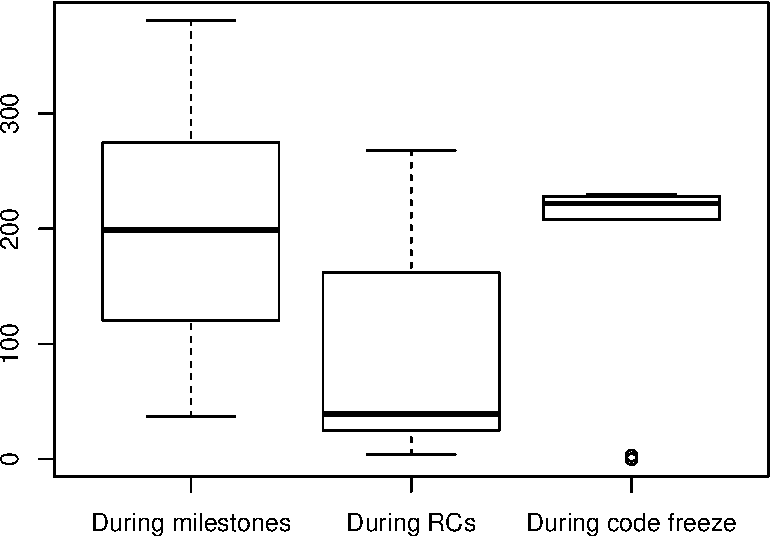
\includegraphics[width=0.60\textwidth,keepaspectratio]
		{chapters/chapter4/figures/eclipse_phases_boxplot.pdf}
	}

	\subfloat[Firefox]{
		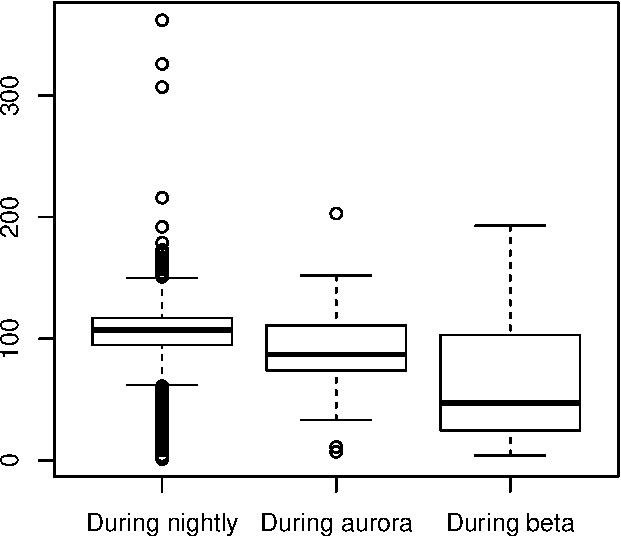
\includegraphics[width=0.60\textwidth,keepaspectratio]
		{chapters/chapter4/figures/firefox_phases_boxplot.pdf}
	}

	\subfloat[ArgoUML]{
		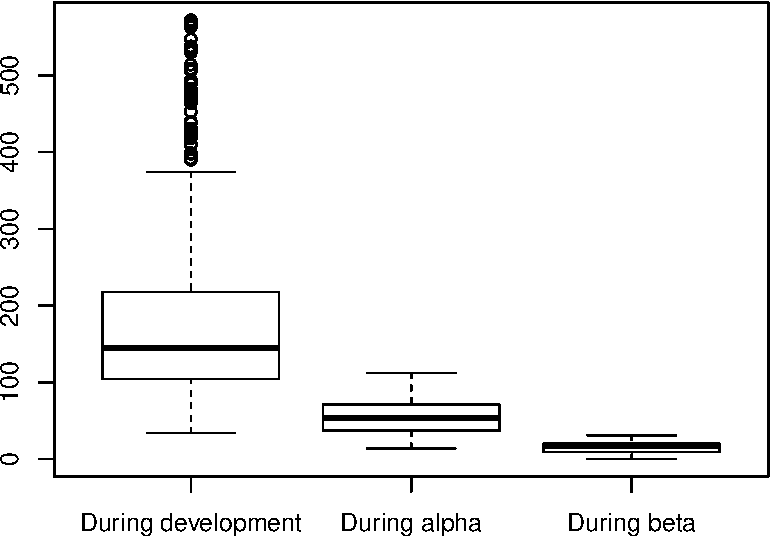
\includegraphics[width=0.60\textwidth,keepaspectratio]
		{chapters/chapter4/figures/argouml_phases_boxplot.pdf}
	}

	\caption{\textbf{delivery delay during release
		cycle stages.} Issues that are addressed during more stable stages of a release cycle
	are likely to have a shorter delivery delay}
	\label{ch4:fig:cycle_phases}
\end{figure}


\begin{table}
	\footnotesize
	\centering
	\caption{\textbf{Statistical analysis.} An overview of the $p$-$values$
		and $deltas$ that are observed during our statistical analyses.
		\label{ch4:tbl:statisticalrq2}
	}
	\resizebox{\textwidth}{!}{
		\begin{tabular}{llrrr}
			\hline 
			& \textbf{Comparison} & \textbf{Kruskal-Wallis} ($p$) &
			\textbf{Dunn} ($p.adjusted$) & \textbf{Effect-size} ($delta$)\tabularnewline
			\hline 
			\multirow{3}{*}{\textbf{Eclipse}} & Milestones vs RCs &
			\multirow{3}{*}{$1.87 \times 10^{-51}$} & $1.47 \times 10^{-52}$ & (large) $0.63$\tabularnewline
			\cline{2-2} \cline{4-5} & RCs vs Code freeze &  & $0.56$ & Not apply\tabularnewline \cline{2-2} \cline{4-5} & Milestones vs Code freeze &  & $0.02$ & (negligible) $0.09$\tabularnewline
			\hline 
			\multirow{3}{*}{\textbf{Firefox}} & Nightly vs Aurora &
			\multirow{3}{*}{$2.99 \times 10^{-76}$} & $5.07 \times 10^{-49}$ &
			(medium) $0.40$\tabularnewline
			\cline{2-2} \cline{4-5} 
			& Aurora vs Beta &  & $1.72 \times 10^{-03}$ & (medium) $0.40$\tabularnewline
			\cline{2-2} \cline{4-5} 
			& Nightly vs Beta &  & $1.43 \times 10^{-31}$ & (large) $0.57$\tabularnewline
			\hline 
			\multirow{3}{*}{\textbf{ArgoUML}} & Development vs Alpha
			& \multirow{3}{*}{$2.73 \times 10^{-135}$} & $7.24 \times 10^{-89}$
			& (large) $0.94$\tabularnewline
			\cline{2-2} \cline{4-5} 
			& Alpha vs Beta &  & $3.98 \times 10^{-09}$ & (large) $0.98$\tabularnewline
			\cline{2-2} \cline{4-5} 
			& Development vs Beta &  & $1.14 \times 10^{-78}$ & (large) $0.99$\tabularnewline
			\hline 
		\end{tabular}
	}
\end{table}

\noindent\textit{\textbf{Many issues that are prevented from integration are
addressed well before the code freeze stage of their respective release cycle.}} We
compute the {\em fix timing} metric that we present in \hyperref[rq1]{RQ1}.
However, instead of counting the number of days until an upcoming release, we
count the number of days until an upcoming code freeze stage
(\hyperref[ch4:eq:fixtiming2]{Equation}~\ref{ch4:eq:fixtiming2}). Our goal is to check
whether addressed issues are being prevented from integration mostly because they
are being addressed too close to a code freeze stage (\ie a period during which
integration of new code changes would likely be minimal).  

\begin{figure} \center 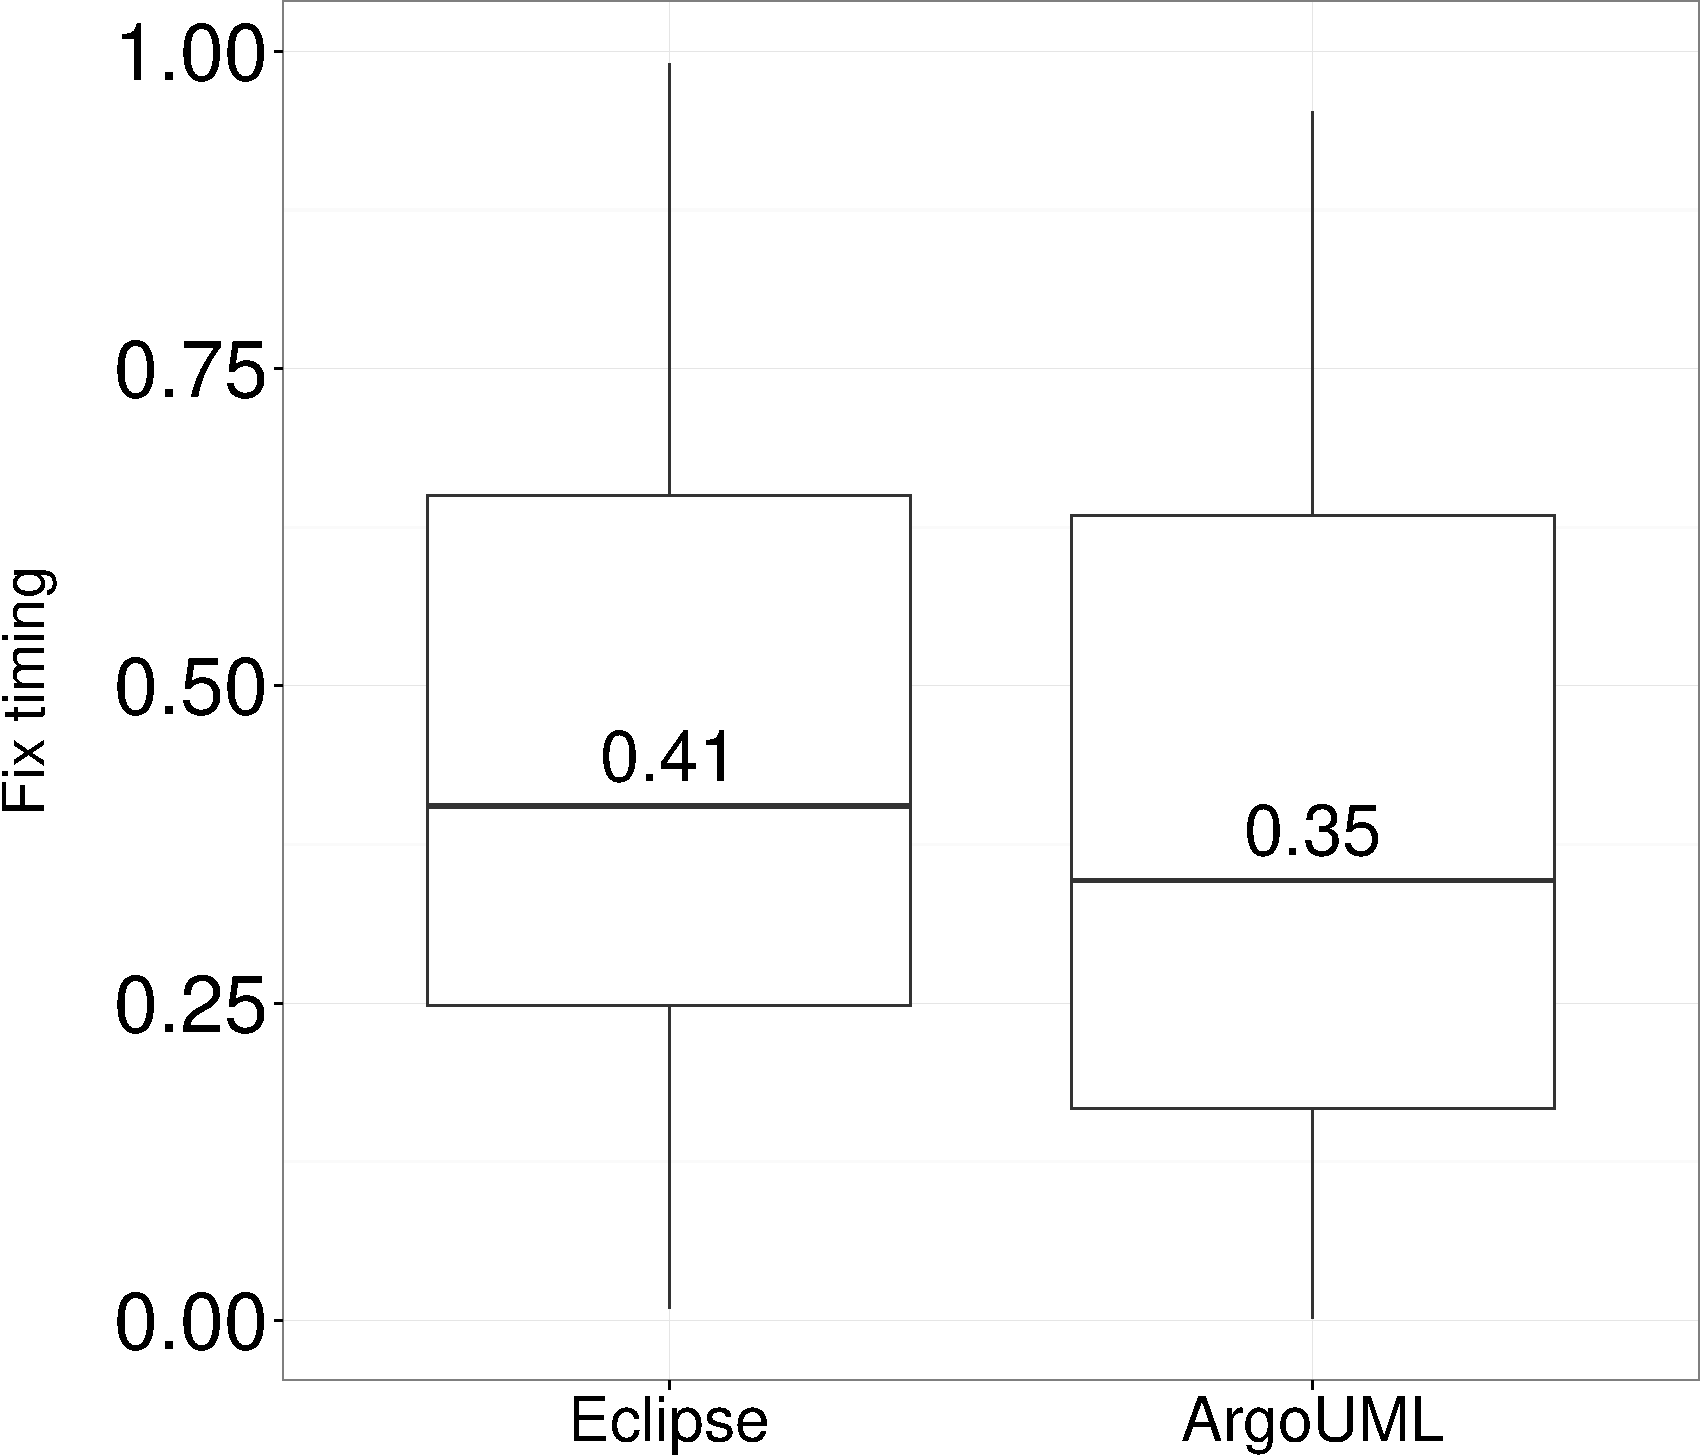
\includegraphics[width=0.60\textwidth,keepaspectratio]
	{chapters/chapter4/figures/as_codefreeze.pdf} \caption{\textbf{{\em Fix timing} values for
		the code freeze period.} The median {\em fix timing} values drop
		from 0.45 and 0.52 to 0.41 and 0.35 in the Eclipse and ArgoUML
projects, respectively. } \label{ch4:fig:codefreeze_allsystems} \end{figure}

In \hyperref[ch4:fig:codefreeze_allsystems]{Figure}~\ref{ch4:fig:codefreeze_allsystems},
we show the {\em fix timing} values for the Eclipse and ArgoUML projects, since
both projects adopt a {\em code freeze} stage. For the Eclipse project, the code
freeze starts after the last release candidate, while for the ArgoUML project,
the code freeze starts at the beginning of the {\em beta} stage (see
\hyperref[ch4:sec:subjects]{Section}~\ref{ch4:sec:subjects}). Naturally, we observe a
drop in the {\em fix timing} values, since both code freeze stages start considerably
before the official release dates. Nevertheless, we observe that even after correcting for
the code freeze stages of the Eclipse and ArgoUML projects, it is unlikely
that addressed issues are being prevented from integration solely because of an approaching code
freeze stage. For instance, although the median {\em fix timing} for the ArgoUML project
dropped from 0.52 to 0.35, the development team would still have 2 months to
integrate an addressed issue---since the median duration of a release cycle in the
ArgoUML project is 180 days.

\conclusionbox{We observe that issues that are addressed during more stable stages of
release cycles are associated with a shorter delivery delay. We also observe
that addressed issues are unlikely to be prevented from integration solely because
they were addressed near an upcoming code freeze stage.}

